\documentclass[10pt]{article}

\usepackage[a4paper, portrait, left=2.25cm, right=2.25cm, top=2cm, bottom=2cm]{geometry}
\usepackage{graphicx}
\graphicspath{ {./pictures} }

\title{COMP3911 Coursework 2}
\author{Boyan Karatotev and Sean Yee}
\date{}

\begin{document}
    \maketitle

    \section{Analysis of Flaws}

        \paragraph{Passwords in plaintext} - the database stores passwords in
        plaintext instead of hashes

        \paragraph{SQL injection} - form inputs are not sanitised and their
        contents are formatted into an SQL query directly instead of using a
        prepared statement or similar and can leak information

        \paragraph{Improper authentication} - the injection allows arbitrary
        authentication

        \paragraph{No encryption} - All communication over the network is in
        plaintext HTTP

        \paragraph{Stored XSS} - patient data is formatted unaltered from the
        database into the webpage allowing HTML in fields to render

        \paragraph{Multiple login with the same credential allowed within the same browser} - The search feature could be used with the same credentials within the same browser simultaneously.


        \subsection{SQL injection in detail}

            One of the easiest flaws to exploit is an SQL injection. It is very
            easy and straightforward to find. There are two instances of it in
            this application - one in the user credential fields and one in the
            patient surname field. Exploiting both is identical with minor
            differences to the impact. As an arbitrary choice, greater focus
            will be placed on the injection in the surname field.

            In essence, this is a command injection vulnerability enabled by
            trusting unvalidated external input. It allows the attacker to
            change the meaning of queries to the database and alter them as he
            sees fit. In the first instance, this enables the attacker to
            bypass the authentication althogether. In the second it enables
            improper information disclosure.

            In the case of the information disclosure, the application does not
            give any facilities to get a list of patients and their personal
            (and very sensitive) information. A lookup should require at least
            knowing their surname. However by submitting \texttt{' OR 1=1; --}
            as the surname field completely bypasses that and returns a
            complete dump of the patients table. A screenshot of this can be
            seen in figure \ref{injection}. Further, the attacker can craft a
            more complex query (for example \texttt{' OR 1=1 LIMIT 1; --}) to
            perform more complex actions like avoid detection.

            \begin{figure}[h!]
                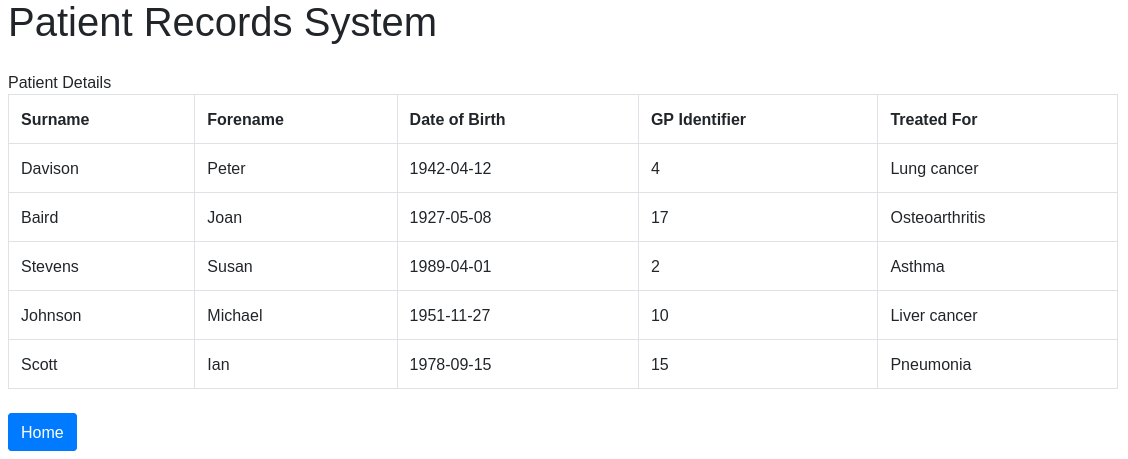
\includegraphics[width=\textwidth]{injection}
                \caption{Result of SQL injection to show all entries in the patients table}
                \label{injection}
            \end{figure}

            This vulnerability was discovered by looking at the source code.
            The queries at the top have \texttt{\%s} placeholders instead of
            \texttt{?} placeholders and are later used in a simple
            \texttt{String.format} operation. Finally, the surname parameter is
            passed verbatim from the request without validation or any scaping.
            This is a textbook example of an SQL injection and very easy to
            find.

            The injection in the authentication fields was found and exploited
            the same way.

            \subsection{Potential for Man in the middle attack (MITM)
            The vulnerbility was discovered by testing to see if the application was
            able to perform the search function with the same account credentials while there was another session running concurrently, which waswas successful.

            This shows the potential for an attacker to perform MITM attack by hijacking the session since there is the absence of SSL or session ID, and also given that form field of the password is sent in plaintext,the attacker would be able to easily impersonate a legitimate user and perform undesired actions by intercepting the connection between the user and application server.

            The threat is further heightened as there is also no session timeout  hence, once the attacker successfully manages to capture the session there is little to no safeguards in place.

    \section{Fixes implemented}
        % Write a short (maximum of one A4 page) summary of the changes that
        % you have made, explaining in each case how it has fixed the problem

        \subsection{SQL injection}

            The fix is simple - replace the \texttt{java.sql.Statement}s with
            \texttt{java.sql.PreparedStatemt}s. To do this, the query templates
            need to have their \texttt{\%s} replaced with a \texttt{?} and then
            have them initialised at startup. Now instead of formatting the
            strings directly, the user input is given to the prepared statement
            with \texttt{setString} and executed and handled as before. This
            has to be done in both the \texttt{authenticated()} and
            \texttt{searchResults()}} methods.

            This fixes the vulnerability because the unvalidated user input is
            no longer formatted into the query. Instead, the query is sent to
            the database at application initialision which returns a compiled
            version which is used to handle requests in its place. This way the
            user input is never part of the query itself but is rather sent as
            a parameter to the precompiled qeuery separately. Further, since
            the statement is precompiled, there is no way for a text based
            attack (but not others like the compiled format).


        \subsection{MITM attack}

          The fix for the vulnerbility after considering various options such as  creating a token/ session ID to using SSL , the best option sought out was to store the passwords as hashes in the database using SHA256 which is achieved using Java's Messagedigest class that performs the hashing on the passwords that are to be stored. As this would firstly eliminate the issue of easy compromise due to being stored in plaintext. Secondly, by matching against using a hash function for the password it would provide another layer of security against attackers as they would need to figure out the hash function before being able to get the password.

\end{document}
